%template for producing IEEE-format articles using LaTeX.
%written by Matthew Ward, CS Department, Worcester Polytechnic Institute.
%use at your own risk.  Complaints to /dev/null.
%make two column with no page numbering, default is 10 point



\documentclass[twocolumn]{article}
\usepackage[pdftex]{graphicx}
\pagestyle{empty}
\usepackage[utf8]{inputenc} 
\usepackage[round,sort,comma]{natbib}

\renewcommand*\familydefault{\sfdefault} 
\usepackage[scaled]{helvet} %para usar helvetica
\renewcommand\familydefault{\sfdefault} 
\usepackage[T1]{fontenc}
\usepackage{hyperref}

%set dimensions of columns, gap between columns, and space between paragraphs
\setlength{\textheight}{8.75in}
\setlength{\columnsep}{2.0pc}
\setlength{\textwidth}{6.8in}
%\setlength{\footheight}{0.0in}
\setlength{\topmargin}{0.25in}
\setlength{\headheight}{0.0in}
\setlength{\headsep}{0.0in}
\setlength{\oddsidemargin}{-.19in}
\setlength{\parindent}{1pc}

%I copied stuff out of art10.sty and modified them to conform to IEEE format

\makeatletter
%as Latex considers descenders in its calculation of interline spacing,
%to get 12 point spacing for normalsize text, must set it to 10 points
\def\@normalsize{\@setsize\normalsize{12pt}\xpt\@xpt
\abovedisplayskip 10pt plus2pt minus5pt\belowdisplayskip \abovedisplayskip
\abovedisplayshortskip \z@ plus3pt\belowdisplayshortskip 6pt plus3pt
minus3pt\let\@listi\@listI} 

%need an 11 pt font size for subsection and abstract headings
\def\subsize{\@setsize\subsize{12pt}\xipt\@xipt}

%make section titles bold and 12 point, 2 blank lines before, 1 after
\def\section{\@startsection {section}{1}{\z@}{24pt plus 2pt minus 2pt}
{12pt plus 2pt minus 2pt}{\large\bf}}

%make subsection titles bold and 11 point, 1 blank line before, 1 after
\def\subsection{\@startsection {subsection}{2}{\z@}{12pt plus 2pt minus 2pt}
{12pt plus 2pt minus 2pt}{\subsize\bf}}
\makeatother

\usepackage{graphicx}  
\newcommand{\imgdir}{doc-img} 
\graphicspath{{\imgdir/}} 
\usepackage{amsmath}


\begin{document}


%don't want date printed
\date{}

%make title bold and 14 pt font (Latex default is non-bold, 16 pt)
\title{\Large\bf Análisis de liberación de catecolaminas en células cromafines de ratón mediante Amperometría}

%for single author (just remove % characters)
\author{J. Palma-Espinosa \\
  Laboratorio de Neurociencia Computacional - CNScLAB \\
  Universidad Valparaíso. Valparaíso, Chile \\
  javier.palma@cinv.cl}
 
%for two authors (this is what is printed)
%\author{\begin{tabular}[t]{c@{\extracolsep{8em}}c}
%  I. M. Author	& M. Y. Coauthor \\
% \\
%  My Department & Coauthor Department \\
%  My Institute & Coauthor Institute \\
%  City, ST~~zipcode	& City, ST~~zipcode
%\end{tabular}}

\maketitle

%I don't know why I have to reset thispagesyle, but otherwise get page numbers
\thispagestyle{empty}

\subsection*{\centering Abstract}
%IEEE allows italicized abstract
{\em
En un organismo pluricelular, las células deben interpretar las numerosas señales que reciben desde otras células.  Durante este proceso de señalización, la célula que porta el mensaje, libera moléculas mensajeras  al medio extracelular, en un proceso llamado exocitosis. Para estudiar la exocitosis, se suelen emplear cultivos de líneas celulares, siendo uno de los más utilizados las células cromafinas de la glándula adrenal.  Empleando amperometría, se midieron los eventos de exocitosis y se analizarón las variables que podrían estar mediando en este proceso, mostrando que la exocitosis se provoca mediante dos vías diferentes.
{\bf Keywords: Amperometría, célula cromafin, exocitosis, pyhon}
}


\section{Introducción}
En un organismo pluricelular, las células deben interpretar las numerosas señales que reciben desde otras células\citep{alberts2006introduccion}. Estas señales, generan respuestas químicas que permiten coordinar no sólo su propio comportamiento, sino también generar respuestas a una escala superior, que permita la supervivencia de dicho organismo \citep{jarukanont2015vesicle}.
Esta cadena de interpretación y generación de señales suele realizarse por vías químicas, mediante la exocitosis regulada de moléculas bioquímicas\citep{evanko2005primer, aspinwall1999comparison}, tales como catecolaminas, serotonina y péptidos \citep{mosharov2005analysis}, que desencadenarán la respuesta deseada en la célula blanco, en particular.
Durante este proceso, la célula que porta el mensaje, libera moléculas mensajeras  al medio extracelular, en un proceso llamado exocitosis\citep{gonzalez2010association}, el cual se produce cuando vesículas portadoras de las moléculas señalizadoras, generan un poro de fusión entre las membranas de la vesícula y la célula\citep{amatore2009quantitative,oleinick2013vesicular}, generando un flujo de tales moléculas hacia el medio extracelular, o espacio sináptico en el caso de neuronas.\\
{\bf Modelos de Exocitosis.\\}
Actualmente, se conocen tres modelos por los cuales se produce la exocitosis de moléculas mensajeras: Colapso-fusión completa, kiss and run y exocitosis compuesta.  
El modelo de \textit{exocitosis de fusión completa} propone que la vesícula transportadora comienza a fusionarse con la membrana celular, generando un espacio , de forma tal que esta fusión provoca una liberación de las moléculas señalizadoras hacia el medio extracelular, mientras que el modelo de \textit{exocitosis compuesta} establece que la fusión a la membrana celular se realiza por complejos vesícula-vesícula fusionados previamente\citep{wu2014exocytosis}.  
El modelo de \textit{kiss and run} se plantea como una fusión no convencional entre las vesículas secretoras y los espacios de membrana que liberarán su contenido intravesicular. Su característica principal es que la vesícula mantiene, en términos generales, su forma, realizando sólo una pequeña integración a la membrana celular, para luego de liberar una pequeña cantidad de componentes señalizadores, es capaz de retirarse de la membrana y volver a lúmen celular\citep{alabi2013perspectives}.\\
{\bf Células cromafinas como modelo de estudio de exocitosis.\\}
Para estudiar la exocitosis, se suelen emplear cultivos de líneas celulares\citep{O'Neill-1994}, tales como células cromafinas de la glándula adrenal\citep{bader2002exocytosis,wightman1991temporally},  o mastocitos para el estudio de serotonina\citep{reynier1997ne} . 
Para el estudio de liberación de catecolaminas se utilizan cultivos de células adrenales cromafinas, ya sean bovinas o de roedores. El origen en el neuroectodermo, junto con sus similaridades con las neuronas del sistema simpático, permiten que las células cromafinas sean un buen modelo para la exocitosis de catecolaminas.  Adicionalmente, debido a su estabilidad en el cultivo, preservando  las propiedades de la glándula \textit{in vivo} este tipo de células se ha convertido en el modelo más utilizado\citep{bader2002exocytosis,leszczyszyn1991secretion,wightman1991temporally}. \\
{\bf Amperometría y mediciones de liberación de neurotransmisores.\\}
El grupo de Wightman\citep{leszczyszyn1990nicotinic,leszczyszyn1991secretion, mosharov2005analysis}, mostraron que la utilización de electrodos de fibra de carbono para la detección de la secreción de catecolaminas liberadas por células cromafinas, es farmacológicamente indistinto de las encontradas en múltiples preparaciones celulares, reportadas previamente por varios laboratorios\citep{phillips1983visualization,viveros1969quantal}.  En esta técnica, denominada amperometría, se detecta la secreción de catecolaminas a través de dicho electrodo,  mediante una corriente electroquímica, medida al colocar el electrodo en la superficie de la célula secretora y registrando  la  actividad exocitótica debido a la oxidación de los neurotransmisores liberados en el medio extracelular.  Esta actividad se observa a través de \textit{spikes} o espigas electroquímicas de corriente, generadas por una estimulación externa a la célula en estudio.

\begin{figure*}[h!]
\centering
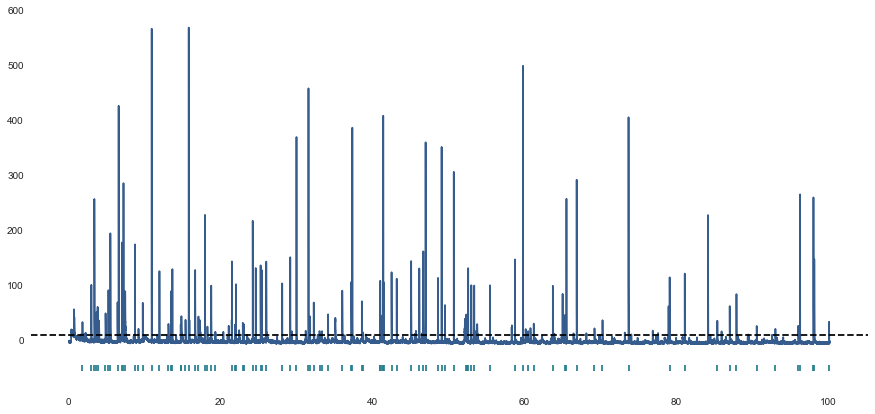
\includegraphics[scale=0.4]{recording.png} 
%\caption{Simulated time series with AWGN (a) and AWGN + impulsive noise (b). Extracted from \citep{cheffena2016propagation}}
%\label{fig:impulsive}
\end{figure*}
\begin{figure*}[h!]
\centering
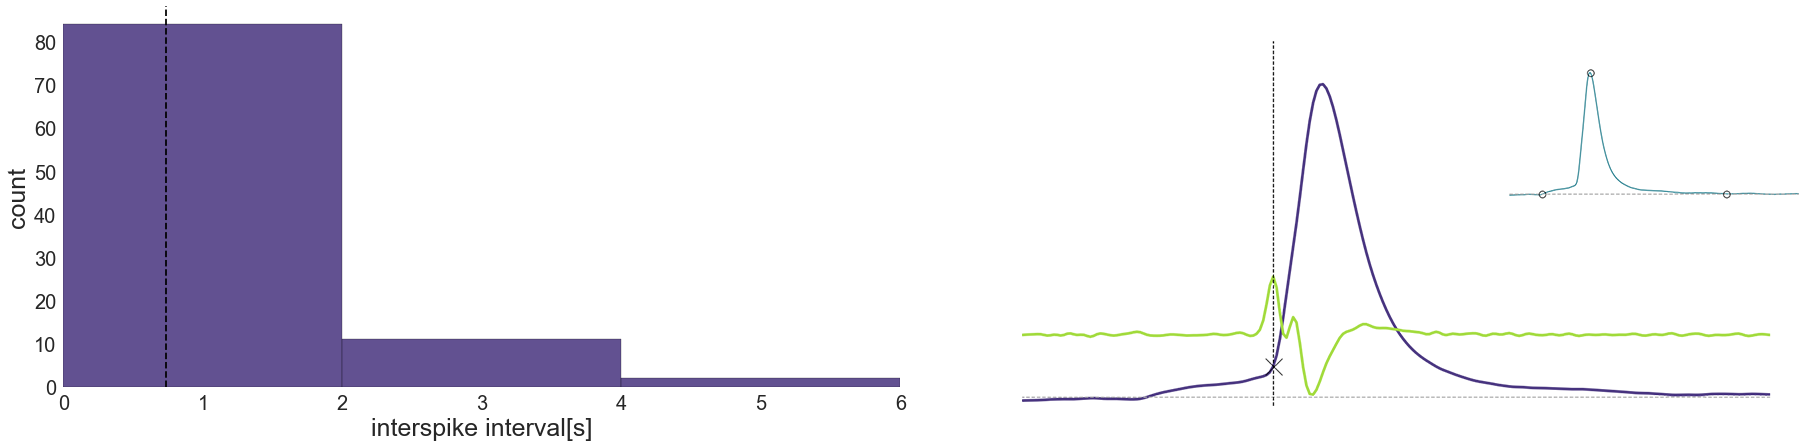
\includegraphics[scale=0.28]{paper_fig2.png} 
\caption{{\bf Escalas temporales de la liberación de neurotransmisores.} (arriba) Registro completo del experimento. Durante los 100 segundos de duración del experimento, se obtuvieron diversos eventos de liberación de neurotransmisores.  La linea muestra el umbral sobre el cual se considerarán los eventos.  Al pie del gráfico, se muestran los eventos que fueron considerados para el análisis ($I_{max}>3pA$;$t_{1/2}>3ms$).
(abajo-izquierda) Histograma del ISI. La linea negra marca la media de la distribución. (abajo-derecha) Un evento característico.  En lila se muestra el evento, en verde se muestra su segunda derivada.  Se observa que el valor de inicio de la espiga (y que fue tomado también como tiempo de término del pie) coincide con el valor máximo de la segunda derivada del evento, marcado por la linea vertical negra.  La linea gris claro muestra la linea de base. (inset) Mismo evento mostrado a una escala menor.  Se marcaron los puntos de inicio $t_{ie}$, peak $t_{I_{max}}$ y de término del evento $t_{fe}$. La linea gris marca la linea base de la medición.}    
\label{fig:figura1}
\end{figure*}

\section{Materiales y Métodos}
{\bf Cultivo celular.}
Células cromafines de las glándulas adrenales adrenales se aislaron y extrajeron según protocolos previamente descritos\citep{colliver2000quantitative,gonzalez2010association,dominguez2012preparation}.  En resumen, las glándulas adrenales se colocaron directamente en medio de disección células previamente enfriado.  El exceso de grasa de cada glándula fue removido, mientras que los fragmentos medulares se aislaron del tejido cortial en presencia de medio de disección enfriado, con la ayuda de un microscopio de disección.  Todos los fragmentos medulares  se combinaron y almacenaron en hielo, previo a la digestión enzimática.  Posteriormente, se eliminó el medio de disección mediante centrifugación y los fragmentos modulares se resuspendieron en una solución salina que contenía colagenasa y DNAsa como enzimas degradante, durante una hora, a temperatura de 37ºC.  Treinta minutos después de la digestión, se añadió tripsina con EDTA.  Durante el transcurso de la digestión, los fragmentos medulares se trituraron aproximadamente cada 15 minutos.  Al final de la digestión, se eliminaron las enzimas y las células se resuspendieron en medio de cultivo caliente, suplementado con suero bovino fetal.
Luego de la digestión, las células se plaquearon con 4 ml de medio de cultivo sobre placas de cultivo revestidas con poli-D-lisina (Becton Dickinson, Bedford, MA, EE. UU.) y se incubaron a 37ºC con 5\% de CO2. Las células se usaron para experimentos 24 - 48 h después de la siembra.\\
{\bf Detección amperométrica de la exocitosis.}La liberación de catecolaminas se detectó mediante amperometría, como lo muestran estudios previos\citep{gonzalez2010association,evanko2005primer,leszczyszyn1991secretion,wightman1991temporally}.Se crearon electrodos de registro utilizando fibra de carbono(5um de diámetro), insertándolos dentro de capilares de borosilicato(1.5-1.8x100 mm, Kimble Products KIMAX-51º) para posteriormente estirarlos (máx $25\mu m$ diam) y cortarlos.  Luego del proceso de corte, se prepara resina epoxi(1:1 resina:solvente) para sellar la punta de los capilares, calentando la mezcla a 90ºC.  Con la mezcla caliente, se sumerge la punta de los capilares durante 40 segundos y se retira cuidando de no generar burbujas en la resina.  Finalmente, se endurece la resina mediante un protocolo de calentamiento(120 min@200ºC y luego 240min@250ºC).
Los registros electroquímicos se realizaron usando un amplificador de \textit{patch clamp},Axopatch 1C modificado para este fin de acuerdo con las instrucciones del fabricante (Molecular Devices). Las células se colocaron en una cámara de perfusión colocada en la platina de un microscopio invertido y se lavaron en solución amortiguadora Krebs-HEPES (en mM: 140 NaCl, 5 KCl, 2 MgCl2, 2.5 CaCl2, 10 HEPES-NaOH y 10 glucosa, pH 7.4 ) La liberación de catecolamina se estimuló mediante una eyección a presión de 10 s de una solución de $K^+$  100 mM desde una micropipeta situada a 10-15 m de la célula.
Los registros amperometricos fueron entregados pre-procesados. La frecuencia de adquisición fue inferida mediante el ratio de duración del registro versus cantidad de puntos del registro, obteniendose una frecuencia de adquisición de 2.5 kHz. \\
{\bf Análisis de Datos.} Se analizó el registro entregado en formato IGOR (Wavemetrics) mediante un script realizado en Python 3.6.  Previo al análisis, los datos fueron prefiltrados empleando un filtro tipo media móvil, sin embargo, para los análisis posteriores se utilizó el registro sin filtrar. Este script permitió identificar automáticamente las espigas, iniciación y término de los pie, área bajo la curva y $t_{1/2}$ para cada una de las espigas.  Posteriores análisis y gráficos se realizaron empleando un script en jupyter notebook con Python 3.6.  Los scripts utilizados pueden ser descargados en \url{https://github.com/jpalma-espinosa/Amperometria-UV}.
Los peaks con corrientes $I_{peak}<10 pA$, o aquellos que tuviesen un $t_{1/2}<3ms$ fueron excluídos del análisis. Los análisis del pie se restringieron a aquellos que tuviesen una corriente $I_{foot}>3p$, medidos en el punto de máxima amplitud del pie, o aquellos que tuviesen una duración $t_{foot}>3ms$.
\section{Resultados}

\begin{figure*}[h!]
\centering
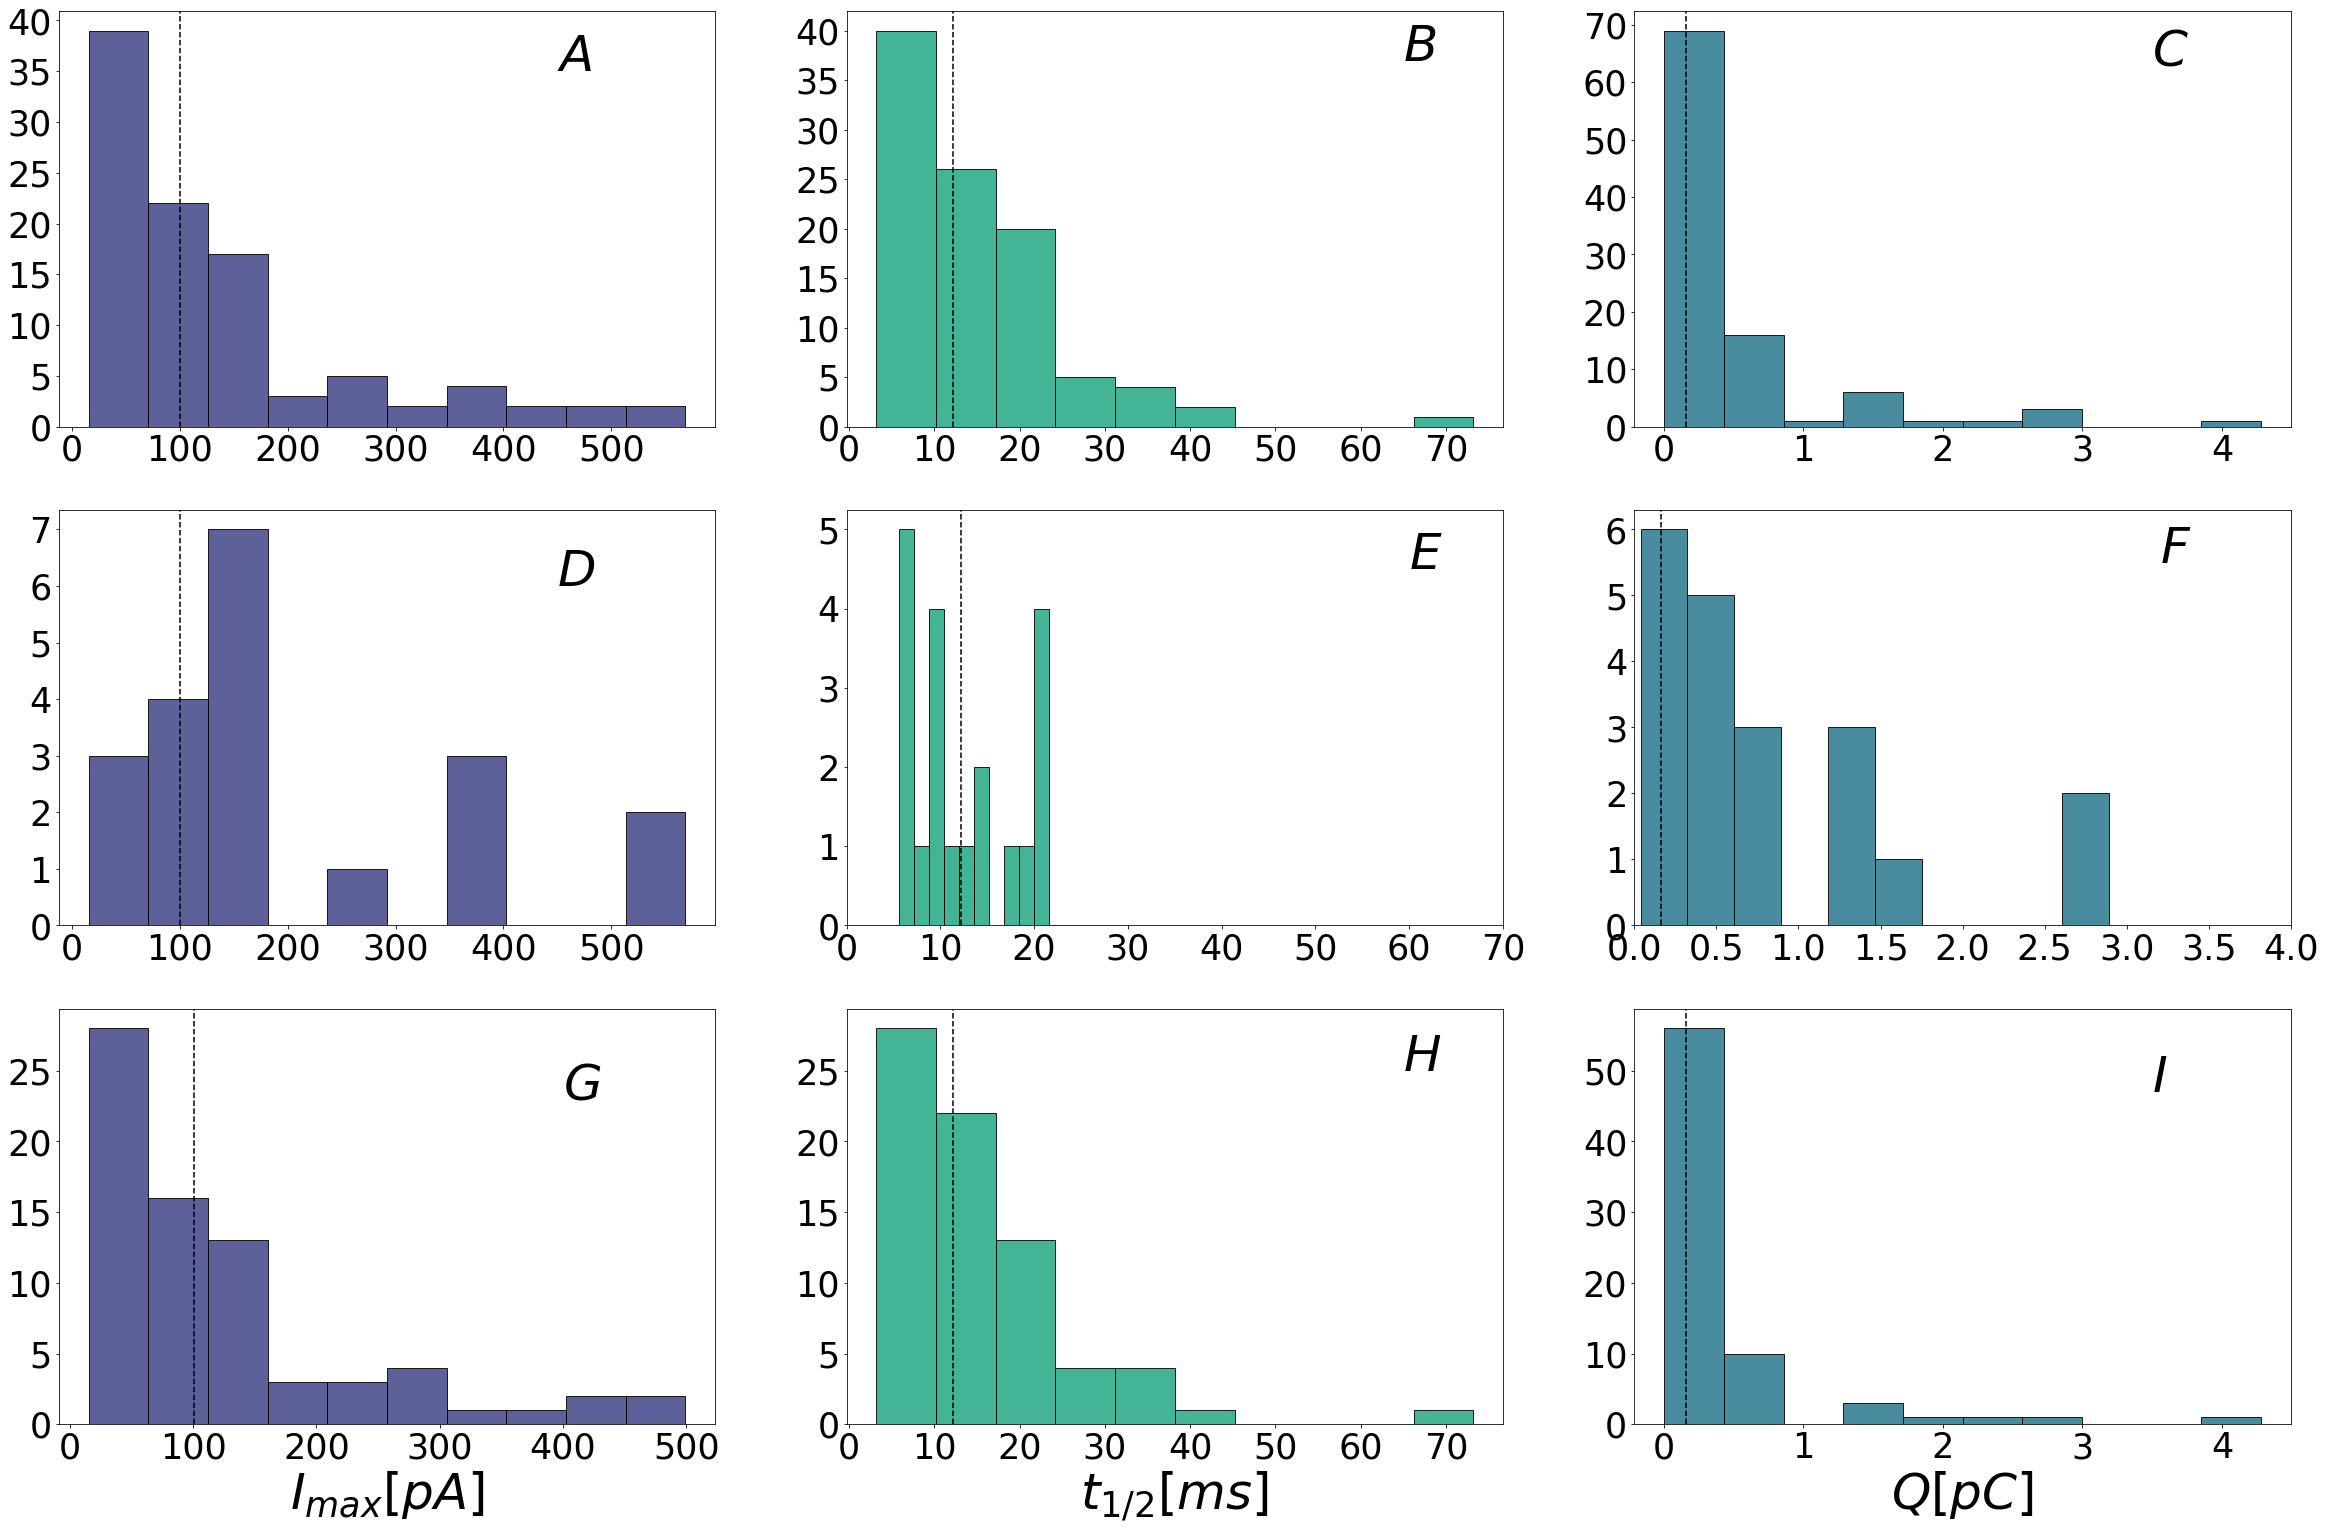
\includegraphics[scale=0.23]{barras.png} 
\caption{Histogramas de $I_{max}$, $t_{1/2}$ y $Q$ para los eventos totales (A,B,C), eventos con pie(D,E,F) y eventos sin pie (G,H,I)}
\label{fig:barras}
\end{figure*}



{\bf Una única célula libera gran cantidad de neurotransmisores.} Para medir la cantidad de catecolaminas liberadas durante el experimento, se calculó el área bajo la curva desde el punto de inicio, $t_{ie}$ al punto de término de un evento $t_{fe}$, entendiendo por evento al fenómeno de pie seguido de una espiga.  Se definió el punto $t_{ie}$ como aquel punto donde, en aquellas espigas que superasen los umbrales seleccionados, se obtenía la mínima amplitud que superase el valor basal.  Análogamente, se definió $t_{fe}$, como aquél punto inmediatamente anterior al nivel basal. El término del pie e inicio de la espiga $t_{fp}$, se definió como el valor donde la segunda derivada tenía su máximo valor\citep{evanko2005primer}.  Para el caso de eventos sin pie, $t_{fp} = t_{ie}$.
La tasa de liberación de catecolaminas se calculó midiendo la diferencia entre los tiempos de $I_{max}$ consecutivos.  De esta manera, pudo obtenerse el \textit{inter spike interval (ISI)} de la célula en cuestión (fig. \ref{fig:figura1}). El ISI medio para la célula en estudio fue de 1.014s.  
Es interesante notar que existe una tasa de liberación constante. Estos resultados concuerdan en parte con lo reportado por otros autores\citep{jarukanont2015vesicle}.  
Además de calcular la tasa de liberación de catecolaminas, se calculó la cantidad total de neurotransmisores liberados durante el experimento.  Para esto, se calculó la cantidad liberada, utilizando $N = \frac{Q}{n*F}$, donde $N$ es la cantidad de moléculas liberadas, $Q$ es el área bajo la curva, medido entre $t_{ie}$ y $t_{fe}$, $n$ es el número de electrones donados por cada molécula oxidada, que para el caso de las catecolaminas es 2, y finalmente $F$ corresponde a la constante de Faraday\citep{evanko2005primer}.\\

{\bf La liberación de neurotransmisores se produce a través de eventos diferentes.}. Para el análisis de liberación de catecolaminas por evento, se separó a los eventos en dos poblaciones: con y sin pie.  Del total de eventos encontrados (N=98), aproximadamente el 75\% de ellos no presentaba el pie previo al spike(N=73). Este resultado es similar a los resultados obtenidos en otros laboratorios \cite{amatore2005correlation,amatore2009quantitative}  Estos eventos sin pie fueron además, separados en aquellos cuya amplitud era superior a $3[pA]$(N=20) e inferior (N=5).

Para medir la contribución de liberación de neurotransmisores al medio extracelular, se calcularon las corrientes máximas del peak, la duración del peak y la cantidad de catecolaminas liberadas, representada mediante el área bajo la curva entre $t_{ie}$ y $t_{fe}$. Los resultados muestran que si bien lo fenómenos con pie presentan una mediana menor de corriente $I_{peak}$ en comparación con aquellos sin pie, un 35\% de ellos presentaron amplitudes de corrientes mayores.  Adicionalmente, los eventos que presentan pie no muestran una distribución distinguible en la duración del peak ($t_{1/2}$) o en la cantidad de catecolaminas liberadas.
Por el contrario, los eventos sin pie presentan una marcada ley de potencias en sus histogramas, destacando su mayor corriente de peak media y su menor $t_{1/2}$(\ref{fig:figura1} A,D y G).\\ \\
\begin{figure*}[h!]
\centering
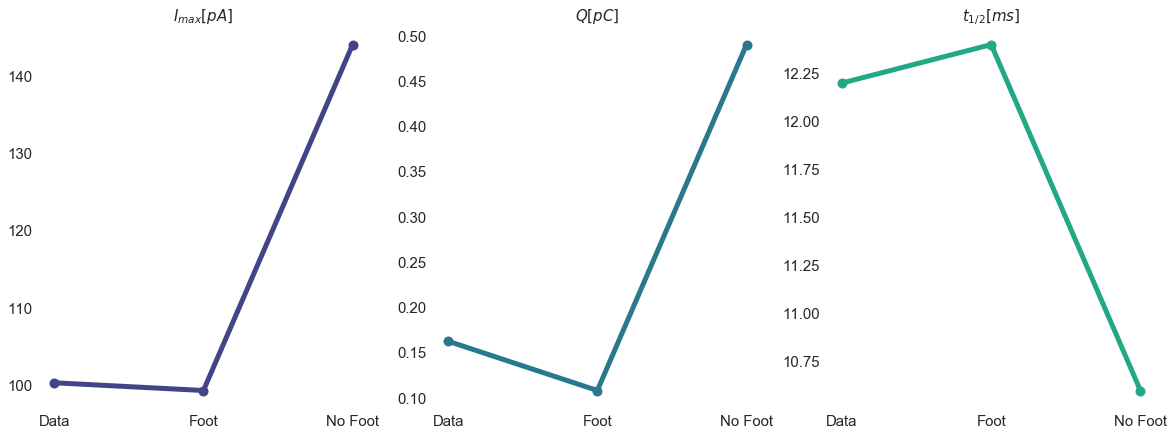
\includegraphics[scale=0.4]{medias.png} 
\caption{Medianas de $I_{max}$, $Q$ y $t_{1/2}$ para los eventos totales(data) eventos con pie(foot) y eventos sin pie (no foot)}
\label{fig:medianas}
\end{figure*}


{\bf Una rápida depleción de las vesículas es el mecanismo principal de liberación de catecolaminas}
Con los datos obtenidos previamente, se observa que la distribución de los fenómenos que no presentan pie es similar a la distribución de la población. En particular, las distribuciones de $t_{1/2}$ y $Q$ son similares para la población completa y la población de espigas sin pie.  Es interesante notar que la mediana de $t_{1/2}$ es menor en el caso de fenómenos sin pie, en contraste con los fenómenos con pie.  Adicionalmente, la mediana de $Q$ es mayor en los fenómenos que presentan pie.  Esto ya ha sido reportado previamente\cite{amatore2009quantitative}, en donde señalan que mientras que el pie se relaciona con el poro de fusión, la espiga está asociada con la fusión de membrana y la exposición del contenido vesicular hacia el medio extracelular.

\section{Discusión}
Los datos analizados permiten estudiar los fenómenos de exocitosis en células cromafines de la glándula adrenal.  Estos fenómenos pueden ser separados en fenómenos con y sin pie, previo a la iniciación de la espiga de liberación\citep{amatore2005correlation}.  
En los datos, se observa que un 25,55\% de los eventos corresponden a eventos que presentan un pie previo a la espiga de liberación, lo que concuerda con resultados reportados previamente\citep{amatore2005correlation, amatore2009quantitative}.  
Una explicación para esto es que el tamaño cuantal muestra dos poblaciones de vesículas dentro de una célula	\citep{grabner2005mouse}.
Adicionalmente, se propone que estas dos poblaciones obedecen a dinámicas diferentes de fusión de vesícula, lo que permite inferir que estas poblaciones son diferentes debido a las dinámicas de fusión de vesículas con la membrana celular\citep{amatore2009quantitative, martens2008mechanisms}.

En resumen, el análisis mediante técnicas de amperometría permite analizar la dinámica de liberación, cantidad de neurotransmisor liberado y establecer principios que podrían explicar el fenómeno de exocitosis.













\bibliographystyle{plainnat}
\bibliography{bibliografia}

\end{document}
